\chapter{Cơ sở lý thuyết.}

\section{Knowledge Graph và Property Graph}

Knowledge Graph là một hướng biểu diễn tri thức trong đó thông tin được tổ chức quanh các thực thể, quan hệ giữa các thực thể và các thuộc tính mô tả chúng. Thay vì chỉ lưu trữ tri thức dưới dạng các đoạn văn bản rời rạc, Knowledge Graph mô hình hóa các đối tượng trong thế giới thực và các liên kết ngữ nghĩa giữa chúng, từ đó hỗ trợ truy vấn, tích hợp dữ liệu và suy luận ở mức cấu trúc hơn so với biểu diễn văn bản thuần túy \cite{hogan2021knowledge}.

Trong bối cảnh khóa luận này, các thực thể có thể là đơn vị, cán bộ, chương trình đào tạo, sự kiện, văn bản, địa điểm hoặc nền tảng số liên quan đến Đại học Công nghệ. Các quan hệ có thể mô tả việc một đơn vị trực thuộc một tổ chức, một cá nhân giữ vai trò trong một đơn vị, một sự kiện được tổ chức bởi một đơn vị, hoặc một thông báo liên quan đến một nhóm đối tượng cụ thể.

Có nhiều cách biểu diễn Knowledge Graph. RDF Graph là một mô hình chuẩn hóa lâu đời, trong đó tri thức thường được biểu diễn bằng các bộ ba subject--predicate--object \cite{rdf11}. Cách biểu diễn này phù hợp với các hệ thống cần liên kết dữ liệu mở, mô tả ontology và khả năng suy luận hình thức.

\begin{figure}[H]
    \centering
    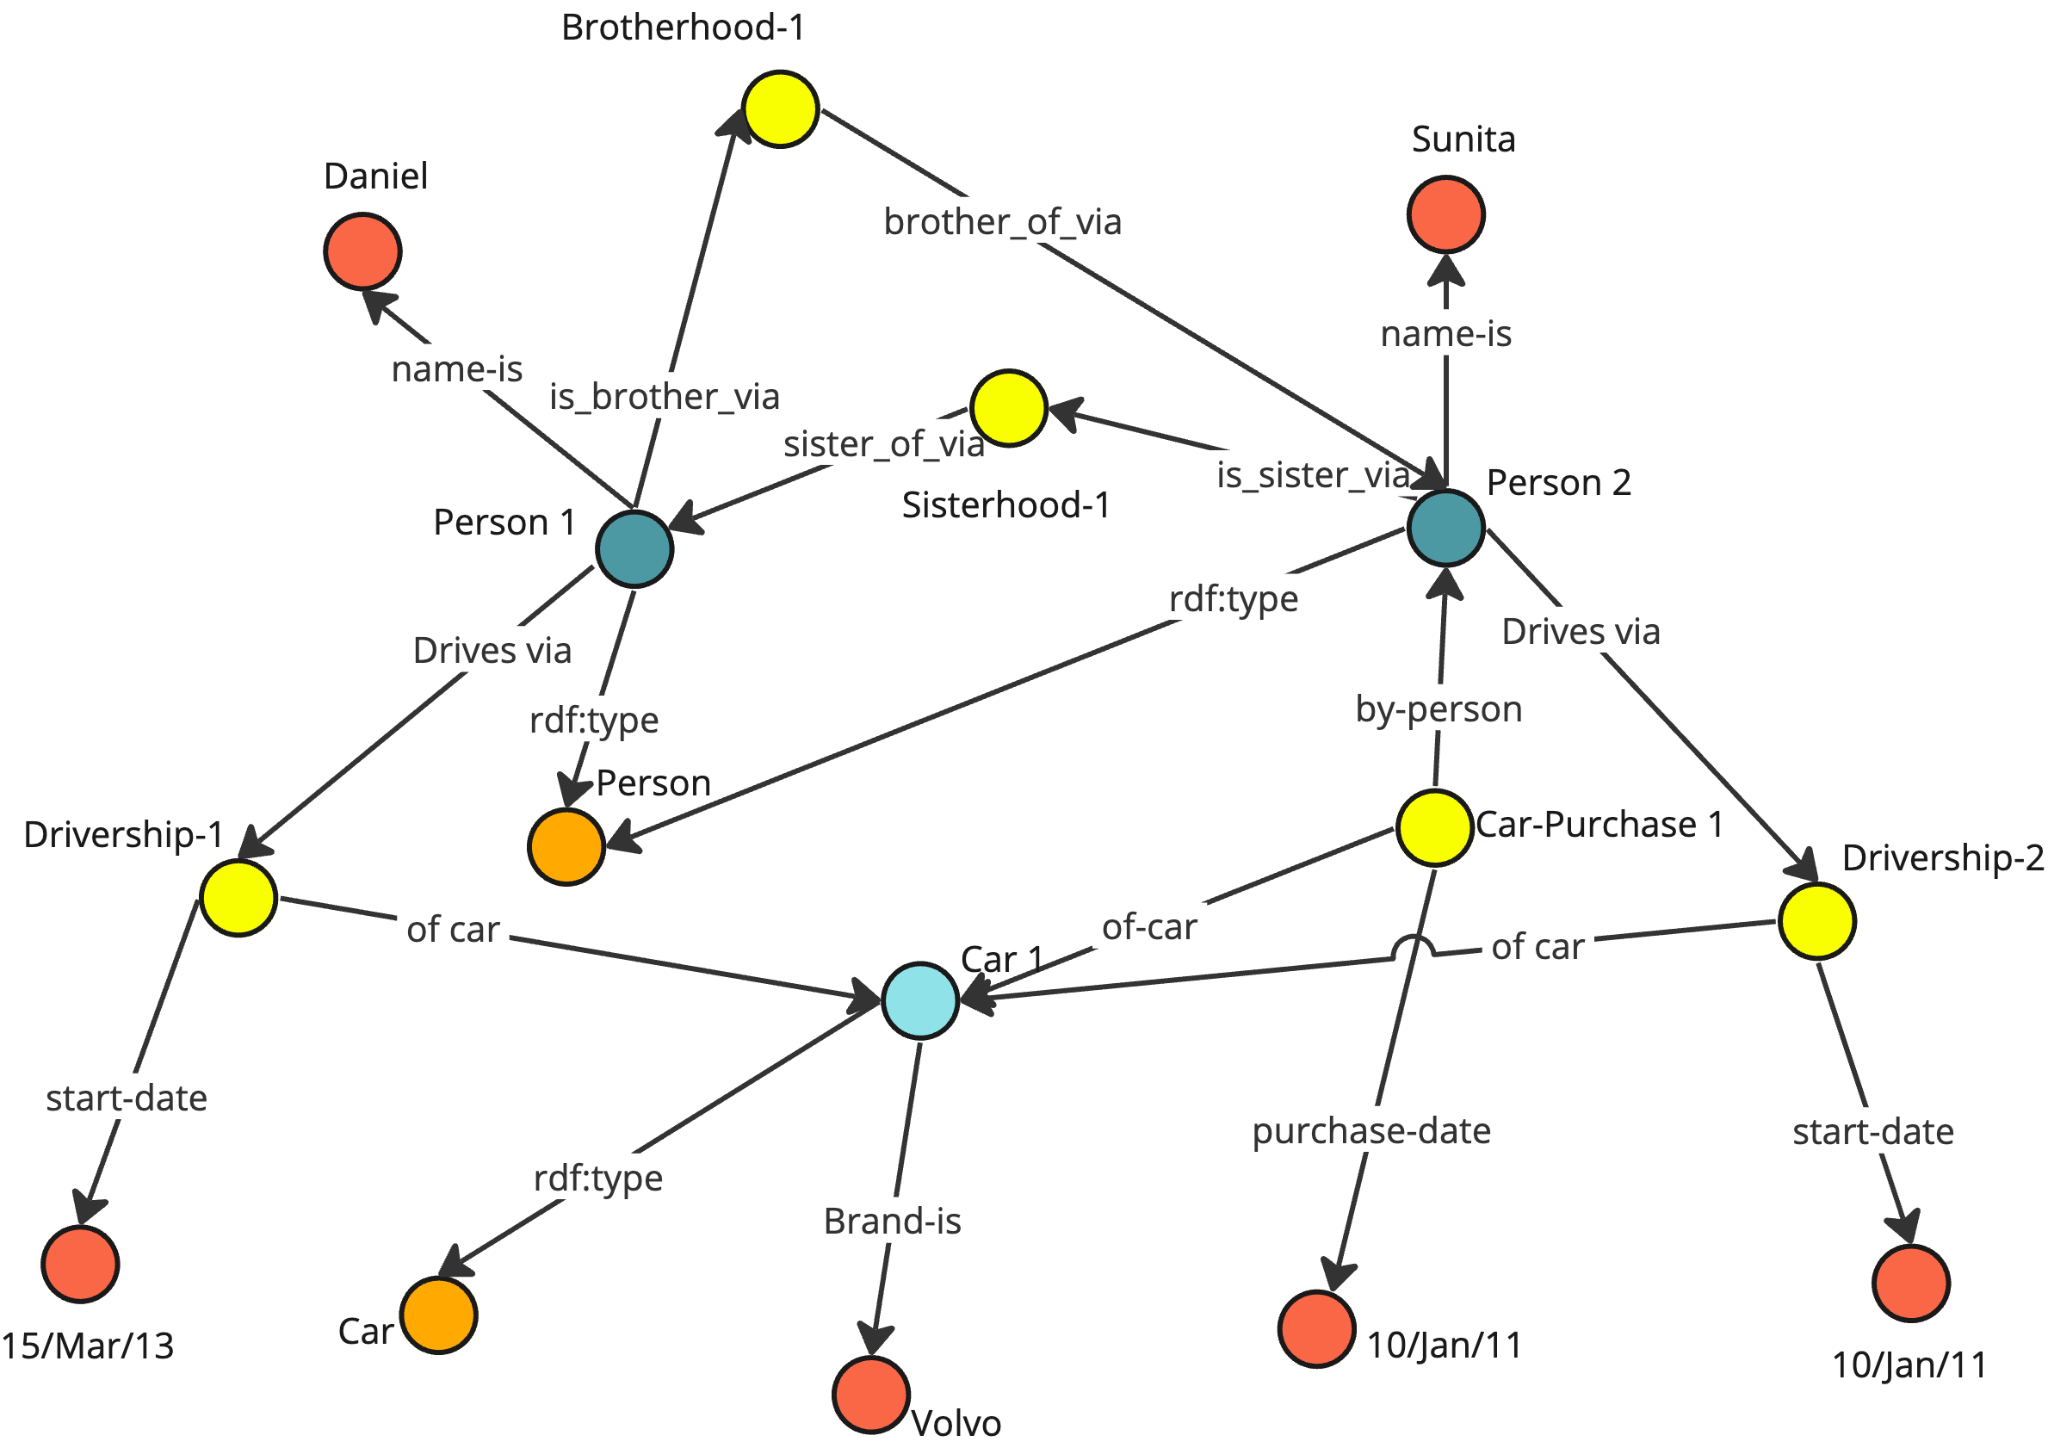
\includegraphics[width=0.82\textwidth]{image/static/rdf-model.png}
    \caption{Ví dụ mô hình RDF Graph, minh họa cách biểu diễn tri thức dưới dạng các bộ ba subject--predicate--object \cite{neo4j_rdf_vs_property}}
    \label{fig:rdf-graph}
\end{figure}

Như minh họa trong Hình \ref{fig:rdf-graph}, mỗi thông tin trong RDF thường được biểu diễn dưới dạng một bộ ba gồm subject, predicate và object. Mô hình này thuận lợi cho việc biểu diễn ngữ nghĩa và liên kết dữ liệu giữa các hệ thống khác nhau.

Bên cạnh RDF, Property Graph là một mô hình phổ biến trong các hệ quản trị cơ sở dữ liệu đồ thị hiện đại. Trong mô hình này, dữ liệu được biểu diễn bằng node và relationship; cả node và relationship đều có thể có nhãn và các thuộc tính dạng khóa--giá trị. Cách tổ chức này thuận tiện cho các bài toán cần truy vấn quan hệ, trực quan hóa graph và phát triển ứng dụng thực tế trên graph database \cite{angles2018property}.

\begin{figure}[H]
    \centering
    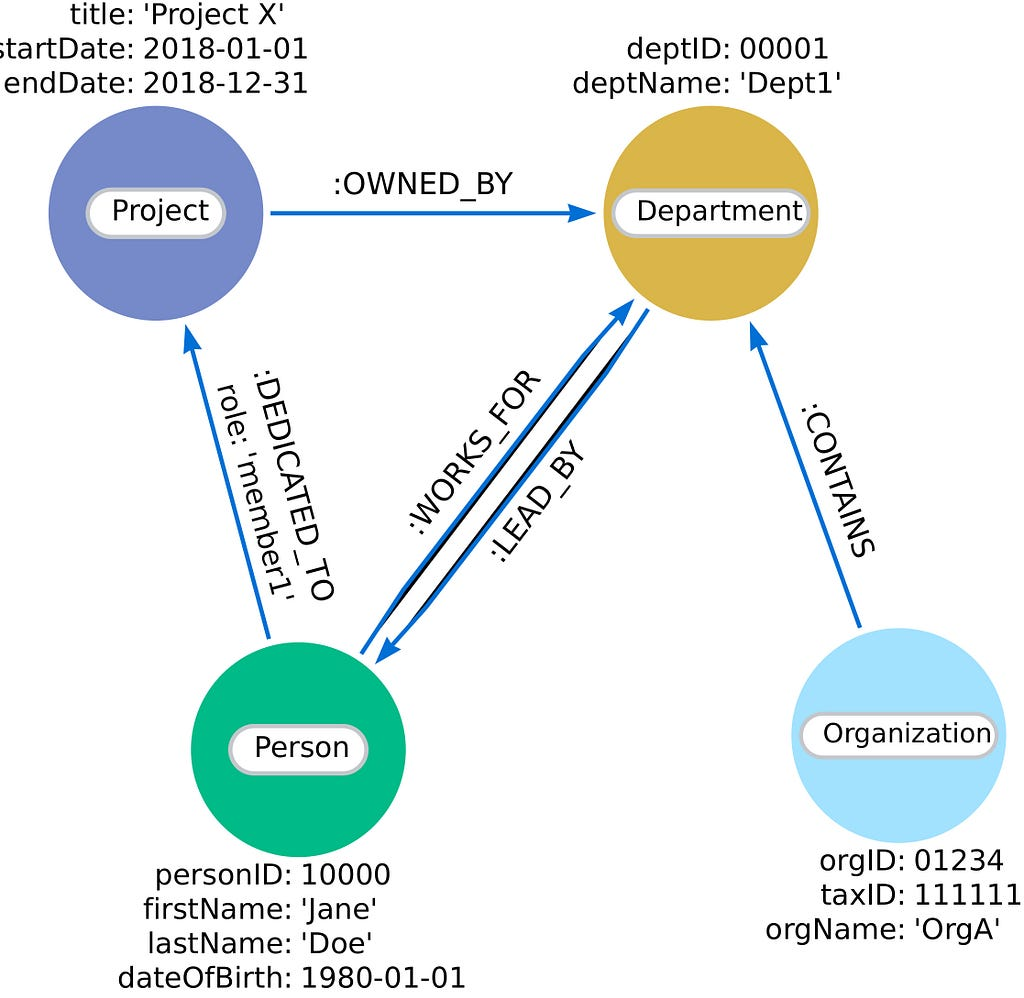
\includegraphics[width=0.78\textwidth]{image/static/property-graph.png}
    \caption{Ví dụ mô hình Property Graph, trong đó node và relationship có thể mang thuộc tính \cite{neo4j_property_graph_image}}
    \label{fig:property-graph}
\end{figure}

Hình \ref{fig:property-graph} cho thấy Property Graph cho phép lưu trữ trực tiếp thuộc tính trên cả node và relationship, từ đó giúp mô hình dữ liệu linh hoạt và gần với cách triển khai trong các graph database như Neo4j.

Trong khóa luận này, Knowledge Graph được triển khai theo hướng Property Graph vì dữ liệu đầu vào có tính bán cấu trúc, quan hệ trong dữ liệu đa dạng và hệ thống cần tích hợp với Neo4j để phục vụ lưu trữ, truy vấn và khai thác trong ứng dụng hỏi đáp. Ngoài ra, Property Graph cũng phù hợp với ngôn ngữ truy vấn Cypher, vốn được thiết kế để thao tác trực tiếp trên các mẫu node--relationship trong graph \cite{francis2018cypher}. Tuy nhiên, việc lựa chọn Property Graph không có nghĩa là bỏ qua vai trò của ontology. Ngược lại, khóa luận vẫn sử dụng schema định hướng để đảm bảo nhãn thực thể, kiểu quan hệ và thuộc tính có tính nhất quán trong quá trình trích xuất và lưu trữ tri thức.

\section{Ontology trong xây dựng Knowledge Graph}

Ontology là một mô hình mô tả các khái niệm, quan hệ và ràng buộc trong một miền tri thức \cite{gruber1993translation}. Trong quá trình xây dựng Knowledge Graph, ontology đóng vai trò như một khung định hướng, hay schema, giúp xác định những loại thực thể nào cần được biểu diễn, các quan hệ nào có thể xuất hiện và những thuộc tính nào cần được lưu trữ \cite{hogan2021knowledge}. Một quy trình phát triển ontology thường bắt đầu từ việc xác định miền và phạm vi, liệt kê các khái niệm quan trọng, tổ chức chúng thành lớp, xác định thuộc tính và ràng buộc của các lớp \cite{noy2001ontology}.

Đối với miền thông tin về Đại học Công nghệ, ontology có thể bao gồm các nhóm khái niệm như tổ chức, đơn vị trực thuộc, con người, chương trình đào tạo, sự kiện, văn bản, học bổng, thông báo và nền tảng số. Việc xác định trước các nhóm khái niệm và kiểu quan hệ này giúp định hướng quá trình trích xuất thông tin bằng LLM theo một schema nhất quán hơn. Nhờ đó, hệ thống có thể giảm tình trạng sinh ra các nhãn thực thể tùy tiện, quan hệ không thống nhất hoặc thông tin thiếu căn cứ trong quá trình trích xuất \cite{pan2024unifying}.

Trong khóa luận này, ontology không được xây dựng theo hướng một ontology hình thức đầy đủ với toàn bộ ràng buộc logic phức tạp. Thay vào đó, ontology được sử dụng như một schema định hướng cho quá trình trích xuất và lưu trữ dưới dạng Property Graph. Cách tiếp cận này phù hợp với mục tiêu thực tế của hệ thống: xây dựng một graph có thể khai thác được cho ứng dụng hỏi đáp, đồng thời vẫn duy trì mức độ nhất quán cần thiết về nhãn thực thể, kiểu quan hệ và thuộc tính \cite{angles2018property}.

\section{Trích xuất thông tin bằng mô hình ngôn ngữ lớn}

Information Extraction là bài toán trích xuất thông tin có cấu trúc từ dữ liệu phi cấu trúc hoặc bán cấu trúc. Trong các hệ thống truyền thống, bài toán này thường được giải quyết bằng rule-based extraction, mô hình học máy có giám sát hoặc các mô hình nhận dạng thực thể. Tuy nhiên, các phương pháp này thường đòi hỏi tập dữ liệu gán nhãn lớn hoặc các tập luật được xây dựng thủ công cho từng miền cụ thể, khiến quá trình thu nhận tri thức tốn nhiều chi phí khi chuyển sang miền dữ liệu mới \cite{ji2021survey}.

Sự phát triển của LLM mở ra khả năng trích xuất tri thức thông qua prompt engineering. Thay vì huấn luyện lại mô hình, hệ thống có thể mô tả nhiệm vụ, định nghĩa schema đầu ra và các ràng buộc trực tiếp trong prompt, sau đó yêu cầu LLM sinh kết quả theo định dạng mong muốn. Cách tiếp cận này đặc biệt phù hợp trong giai đoạn xây dựng nguyên mẫu hoặc với các miền tri thức mà dữ liệu gán nhãn còn hạn chế \cite{pan2024unifying}.

Tuy nhiên, prompt-based Information Extraction cũng đối mặt với nhiều thách thức. LLM có thể sinh sai định dạng, bỏ sót thực thể, tạo ra quan hệ không tồn tại trong văn bản gốc, hoặc sử dụng nhãn không nhất quán. Các lỗi này liên quan trực tiếp đến hiện tượng hallucination, tức mô hình sinh ra nội dung không được hỗ trợ đầy đủ bởi nguồn thông tin đầu vào \cite{ji2023survey}. Đối với tiếng Việt, bài toán càng phức tạp do đặc thù về tên riêng, tên tổ chức, từ ghép và sự đa dạng trong cách viết tắt \cite{nguyen2021phonlp}. Vì vậy, hệ thống cần kết hợp prompt có ràng buộc schema, bước kiểm tra đầu ra và cơ chế xử lý lỗi sau trích xuất.

Trong KGsAuto, LLM được sử dụng để đọc nội dung Markdown và sinh ra các graph fragment gồm danh sách node và relationship ở dạng JSON. Prompt được thiết kế để chỉ dẫn mô hình về nhóm thực thể, kiểu thông tin cần trích xuất, yêu cầu provenance và định dạng đầu ra. Bên cạnh đó, hệ thống sử dụng cơ chế sinh ID tất định dựa trên nội dung thực thể và quan hệ, giúp các artifact sau trích xuất ổn định hơn giữa các lần chạy. Các bước xử lý sau trích xuất tiếp tục phân biệt rõ thực thể đơn lẻ với các cụm thực thể được hợp nhất ở giai đoạn Entity Resolution. Đây là nền tảng cho quy trình xây dựng Knowledge Graph được trình bày chi tiết ở Chương 4.

\section{Entity Resolution trong Knowledge Graph}

Entity Resolution là bài toán phát hiện và hợp nhất các bản ghi hoặc thực thể khác nhau nhưng cùng biểu diễn một đối tượng trong thế giới thực \cite{christen2012data,papadakis2020entity}. Trong Knowledge Graph được trích xuất từ nhiều tài liệu, cùng một thực thể có thể xuất hiện dưới nhiều dạng tên khác nhau. Ví dụ, một tổ chức có thể được gọi bằng tên đầy đủ, tên viết tắt hoặc tên tiếng Anh; một cá nhân có thể xuất hiện cùng với học hàm, học vị hoặc chức vụ; một đơn vị có thể được nhắc đến trong nhiều bài viết với cách viết không hoàn toàn giống nhau.

Nếu không xử lý Entity Resolution, graph sau trích xuất sẽ chứa nhiều node trùng lặp. Điều này làm giảm chất lượng truy vấn, gây phân mảnh thông tin và ảnh hưởng trực tiếp đến chất lượng truy xuất cũng như câu trả lời của hệ thống hỏi đáp. Một câu hỏi về một đơn vị có thể chỉ truy xuất được một phần thông tin nếu các thông tin liên quan bị phân tán ở nhiều node khác nhau. Trong các hệ thống Knowledge Graph, canonicalization và curation là các bước quan trọng để duy trì chất lượng tri thức trong vòng đời của graph \cite{weikum2021machine}.

Các phương pháp Entity Resolution thường kết hợp nhiều kỹ thuật như chuẩn hóa chuỗi, so khớp fuzzy, embedding similarity, blocking, clustering và xác thực bằng mô hình học máy hoặc LLM \cite{papadakis2020entity}. Blocking giúp giảm không gian tìm kiếm các cặp cần so sánh; embedding giúp biểu diễn thực thể trong không gian vector; clustering nhóm các thực thể có khả năng trùng lặp. Các nghiên cứu gần đây cũng cho thấy LLM có tiềm năng hỗ trợ entity matching trong các trường hợp tên gọi phức tạp hoặc cần hiểu ngữ cảnh \cite{peeters2023using}.

Trong khóa luận này, Entity Resolution được xem là một bước độc lập sau trích xuất. Pipeline gồm ba giai đoạn: chuẩn hóa và tạo embedding, blocking và clustering, sau đó xác thực bằng LLM và tổng hợp canonical entity. Để tăng tính minh bạch, hệ thống phân biệt rõ các thực thể không qua hợp nhất với các cụm thực thể đã được hợp nhất. Cách báo cáo này giúp đánh giá chính xác tác động của Entity Resolution thay vì chỉ nhìn vào số lượng thực thể sau xử lý. Quy trình này được trình bày chi tiết trong Chương 5.

\section{Retrieval-Augmented Generation và Graph-based RAG}

Retrieval-Augmented Generation là kiến trúc kết hợp giữa truy xuất thông tin và sinh ngôn ngữ \cite{lewis2020retrieval}. Thay vì để LLM trả lời chỉ dựa trên tham số đã học, hệ thống RAG truy xuất các đoạn tài liệu liên quan đến câu hỏi, đưa các đoạn này vào prompt và yêu cầu LLM sinh câu trả lời dựa trên ngữ cảnh được cung cấp. Cách tiếp cận này giúp cải thiện tính cập nhật của tri thức và giảm nguy cơ sinh câu trả lời không có căn cứ.

RAG truyền thống thường dựa trên semantic search, trong đó tài liệu được chia thành các chunk, chuyển thành embedding và lưu trong vector database. Khi người dùng đặt câu hỏi, hệ thống tìm các chunk gần nhất trong không gian vector. Tuy nhiên, semantic search có hạn chế khi câu hỏi yêu cầu hiểu quan hệ có cấu trúc, truy vấn nhiều bước hoặc tổng hợp thông tin từ nhiều thực thể liên quan \cite{gao2023retrieval}.

Graph-based RAG bổ sung Knowledge Graph vào quá trình truy xuất để hỗ trợ các câu hỏi cần khai thác quan hệ có cấu trúc \cite{edge2024local}. Thay vì chỉ tìm đoạn văn bản gần nghĩa, hệ thống có thể truy xuất node, relationship và path trong graph. Điều này giúp biểu diễn rõ bằng chứng theo quan hệ và hỗ trợ các câu hỏi như “đơn vị nào trực thuộc tổ chức nào”, “ai giữ vai trò gì”, hoặc “sự kiện nào liên quan đến đơn vị nào”.

Trong khóa luận này, hệ thống sử dụng cả semantic search trên văn bản gốc và truy xuất trên Knowledge Graph. Cách kết hợp này cho phép tận dụng ưu điểm của hai nguồn bằng chứng: văn bản gốc cung cấp nội dung chi tiết, trong khi graph cung cấp cấu trúc quan hệ giữa các thực thể. Trên cơ sở đó, hệ thống hỏi đáp được thiết kế với nhiều chế độ truy xuất gồm Semantic Search, Graph Search, Naive Graph RAG và Hybrid RAG. Các chế độ này được trình bày trong Chương 6.

\section{Các công nghệ sử dụng}

Hệ thống KGsAuto sử dụng một số công nghệ chính phục vụ cho các tầng khác nhau của pipeline. Neo4j được sử dụng làm graph database để lưu trữ và truy vấn Knowledge Graph. Neo4j phù hợp với mô hình Property Graph và hỗ trợ truy vấn quan hệ bằng Cypher.

Qdrant được sử dụng làm vector database để lưu trữ embedding của các đoạn văn bản hoặc thực thể. Trong hệ thống, Qdrant phục vụ hai vai trò: hỗ trợ truy xuất markdown chunk trong RAG và hỗ trợ lưu trữ vector trong một số bước của Entity Resolution.

FastAPI được sử dụng để xây dựng backend API và RAG API. Backend cung cấp các chức năng tìm kiếm, truy vấn graph, xem chi tiết thực thể và merge thực thể. RAG API cung cấp giao diện truy vấn cho các chế độ hỏi đáp.

React/Vite được sử dụng để xây dựng frontend cho người dùng cuối. Giao diện hỗ trợ các luồng cơ bản như tìm kiếm, xem trang thực thể, quan sát quan hệ và thao tác merge trong trường hợp cần hiệu chỉnh graph.

Ngoài ra, hệ thống sử dụng Sentence Transformers để tạo embedding và một lớp trừu tượng LLM provider để gọi các mô hình ngôn ngữ khác nhau trong quá trình trích xuất, đối soát thực thể và sinh câu trả lời.
